\documentclass[twoside,twocolumn]{article}

%---package perso---%
\usepackage[utf8]{inputenc}
\usepackage{amsfonts, amsmath, amssymb}
\usepackage[none]{hyphenat}
\usepackage{fancyhdr}
\usepackage{graphicx}
\usepackage{float}
\usepackage[nottoc, notlot, notlof]{tocbibind}
\usepackage{array,multirow,makecell}
\setcellgapes{1pt}
\makegapedcells
\usepackage[table]{xcolor}
\usepackage{import}
\usepackage{tikz}
\usepackage[maxlevel=3]{csquotes}

%---package template---%
\usepackage[sc]{mathpazo} % Use the Palatino font
\usepackage[T1]{fontenc} % Use 8-bit encoding that has 256 glyphs
\linespread{1.05} % Line spacing - Palatino needs more space between lines
\usepackage{microtype} % Slightly tweak font spacing for aesthetics

\usepackage[french]{babel} % Language hyphenation and typographical rules

\usepackage[hmarginratio=1:1,top=32mm,columnsep=20pt]{geometry} % Document margins
\usepackage[hang, small,labelfont=bf,up,textfont=it,up]{caption} % Custom captions under/above floats in tables or figures
\usepackage{booktabs} % Horizontal rules in tables

\usepackage{lettrine} % The lettrine is the first enlarged letter at the beginning of the text

\usepackage{enumitem} % Customized lists
\setlist[itemize]{noitemsep} % Make itemize lists more compact

\usepackage{abstract} % Allows abstract customization
\renewcommand{\abstractnamefont}{\normalfont\bfseries} % Set the "Abstract" text to bold
\renewcommand{\abstracttextfont}{\normalfont\small\itshape} % Set the abstract itself to small italic text

\usepackage{titlesec} % Allows customization of titles
\renewcommand\thesection{\Roman{section}} % Roman numerals for the sections
\renewcommand\thesubsection{\roman{subsection}} % roman numerals for subsections
\titleformat{\section}[block]{\large\scshape\centering}{\thesection.}{1em}{} % Change the look of the section titles
\titleformat{\subsection}[block]{\large}{\thesubsection.}{1em}{} % Change the look of the section titles

\usepackage{fancyhdr} % Headers and footers
\pagestyle{fancy} % All pages have headers and footers
\fancyhead{} % Blank out the default header
\fancyfoot{} % Blank out the default footer
\fancyhead[C]{Travaux Pratique $\bullet$ Février 2022 $\bullet$ 1M8, physique} % Custom header text
\fancyfoot[RO,LE]{\thepage} % Custom footer text

\usepackage{titling} % Customizing the title section

\usepackage{hyperref} % For hyperlinks in the PDF

%----------------------------------------------------------------------------------------
%	TITLE SECTION
%----------------------------------------------------------------------------------------

\setlength{\droptitle}{-4\baselineskip} % Move the title up

\pretitle{\begin{center}\Huge\bfseries} % Article title formatting
\posttitle{\end{center}} % Article title closing formatting
\title{Force de frottement cinétique} % Article title
\author{%
\textsc{Romain Blondel} \\[1ex] % Your name
\normalsize Gymnase Auguste Piccard \\
\and % Uncomment if 2 authors are required, duplicate these 4 lines if more
\textsc{Julien Bricka} \\[1ex]
\normalsize Gymnase Auguste Piccard \\ % Second author's name
\and % Uncomment if 2 authors are required, duplicate these 4 lines if more
\textsc{Jean-Baptiste Freymon} \\[1ex] % Second author's name
\normalsize Gymnase Auguste Piccard \\ % Second author's institution
}
\date{\today} % Leave empty to omit a date
\renewcommand{\maketitlehookd}{%
\begin{abstract}
\noindent Étudier le mouvement de différents blocs de bois glissant sur un plan incliné. Certaines faces des blocs sont recouvertes de plastique ou de toile d'émeri (papier de verre). Le plan incliné peut également être revêtu de ces matières. On choisira les combinaisons suivantes : bois glissant sur bois, bois glissant sur plastique, plastique glissant sur plastique et émeri glissant sur émeri. % Dummy abstract text - replace \blindtext with your abstract text
\end{abstract}
}

%----------------------------------------------------------------------------------------

\begin{document}

% Print the title
\maketitle

%----------------------------------------------------------------------------------------
%	ARTICLE CONTENTS
%----------------------------------------------------------------------------------------

\section{Introduction}
\lettrine[nindent=0em,lines=3]{P}{our} cette expérience, nous essaieront de déterminer le coefficient de frottement via le modèle des lois de Newton. Tout d'abord, il faut mentionner les notions de vitesse ($v = \frac{\Delta d}{\Delta t}$ en $\left[ \frac{m}{s} \right]$), d'accélération ($a = \frac{\Delta v}{\Delta t}$ en $\left[ \frac{m}{s^2} \right]$) et de masse ($m$ en $[Kg]$).La théorie de Newton se base sur les forces : $F = ma$ mesuré en $[N]$, et nous allons nous servir de sa seconde loi : \enquote{Soit un corps de masse m (constante) : l'accélération subie par ce corps [...] est proportionnelle à la résultante des forces qu'il subit, et inversement proportionnelle à sa masse m.} Qui peut être récapitulé comme suit :
$$ \sum_{i} \vec{F_i} = m \vec{a} $$
\begin{figure}[H]
\centering
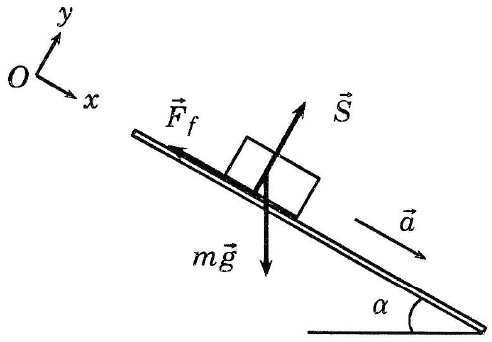
\includegraphics[scale=0.5]{schem_intro.png}
\caption{Schéma des forces dans notre modèle}
\end{figure}
\subparagraph*{}
Dans notre expérience, sachant que $\vec{F_f}$ est la force de frottement, $\vec{S} $ la force de soutient et $ m \vec{g}$ la force de pesanteur, on peut établir via la seconde loi de Newton que 
$$ m \vec{g} + \vec{S} + \vec{F_f} = m \vec{a} $$
D'où, selon $Ox$ :
\begin{equation}\label{eq:ox}
mg \sin \alpha - F_f = m a 
\end{equation}
Selon $Oy$ : 
\begin{equation}\label{eq:oy}
-mg \cos \alpha + S = 0 
\end{equation}
\begin{center}
(\ref{eq:ox}) $\Rightarrow F_f = m(g \sin \alpha - a)$\\
(\ref{eq:oy}) $\Rightarrow S = mg \cos \alpha $
\end{center}
Le but de l'expérience est de vérifier que le coefficient de frottement cinétique $\mu = \frac{F_f}{S}$ ne dépend pas de l'angle, mais uniquement des surfaces mis en présence. Pour observer ce rapport, dans le tableau de résultat, on ne va calculer que l'accélération de ces deux forces car la masse n'influence pas le résultat ; il faut aussi noté que l'on va utiliser $g = 9.81$ $\left[\frac{N}{Kg}\right]$.

%------------------------------------------------

\section{Procédure}
%schéma
\begin{figure}[H]
\centering
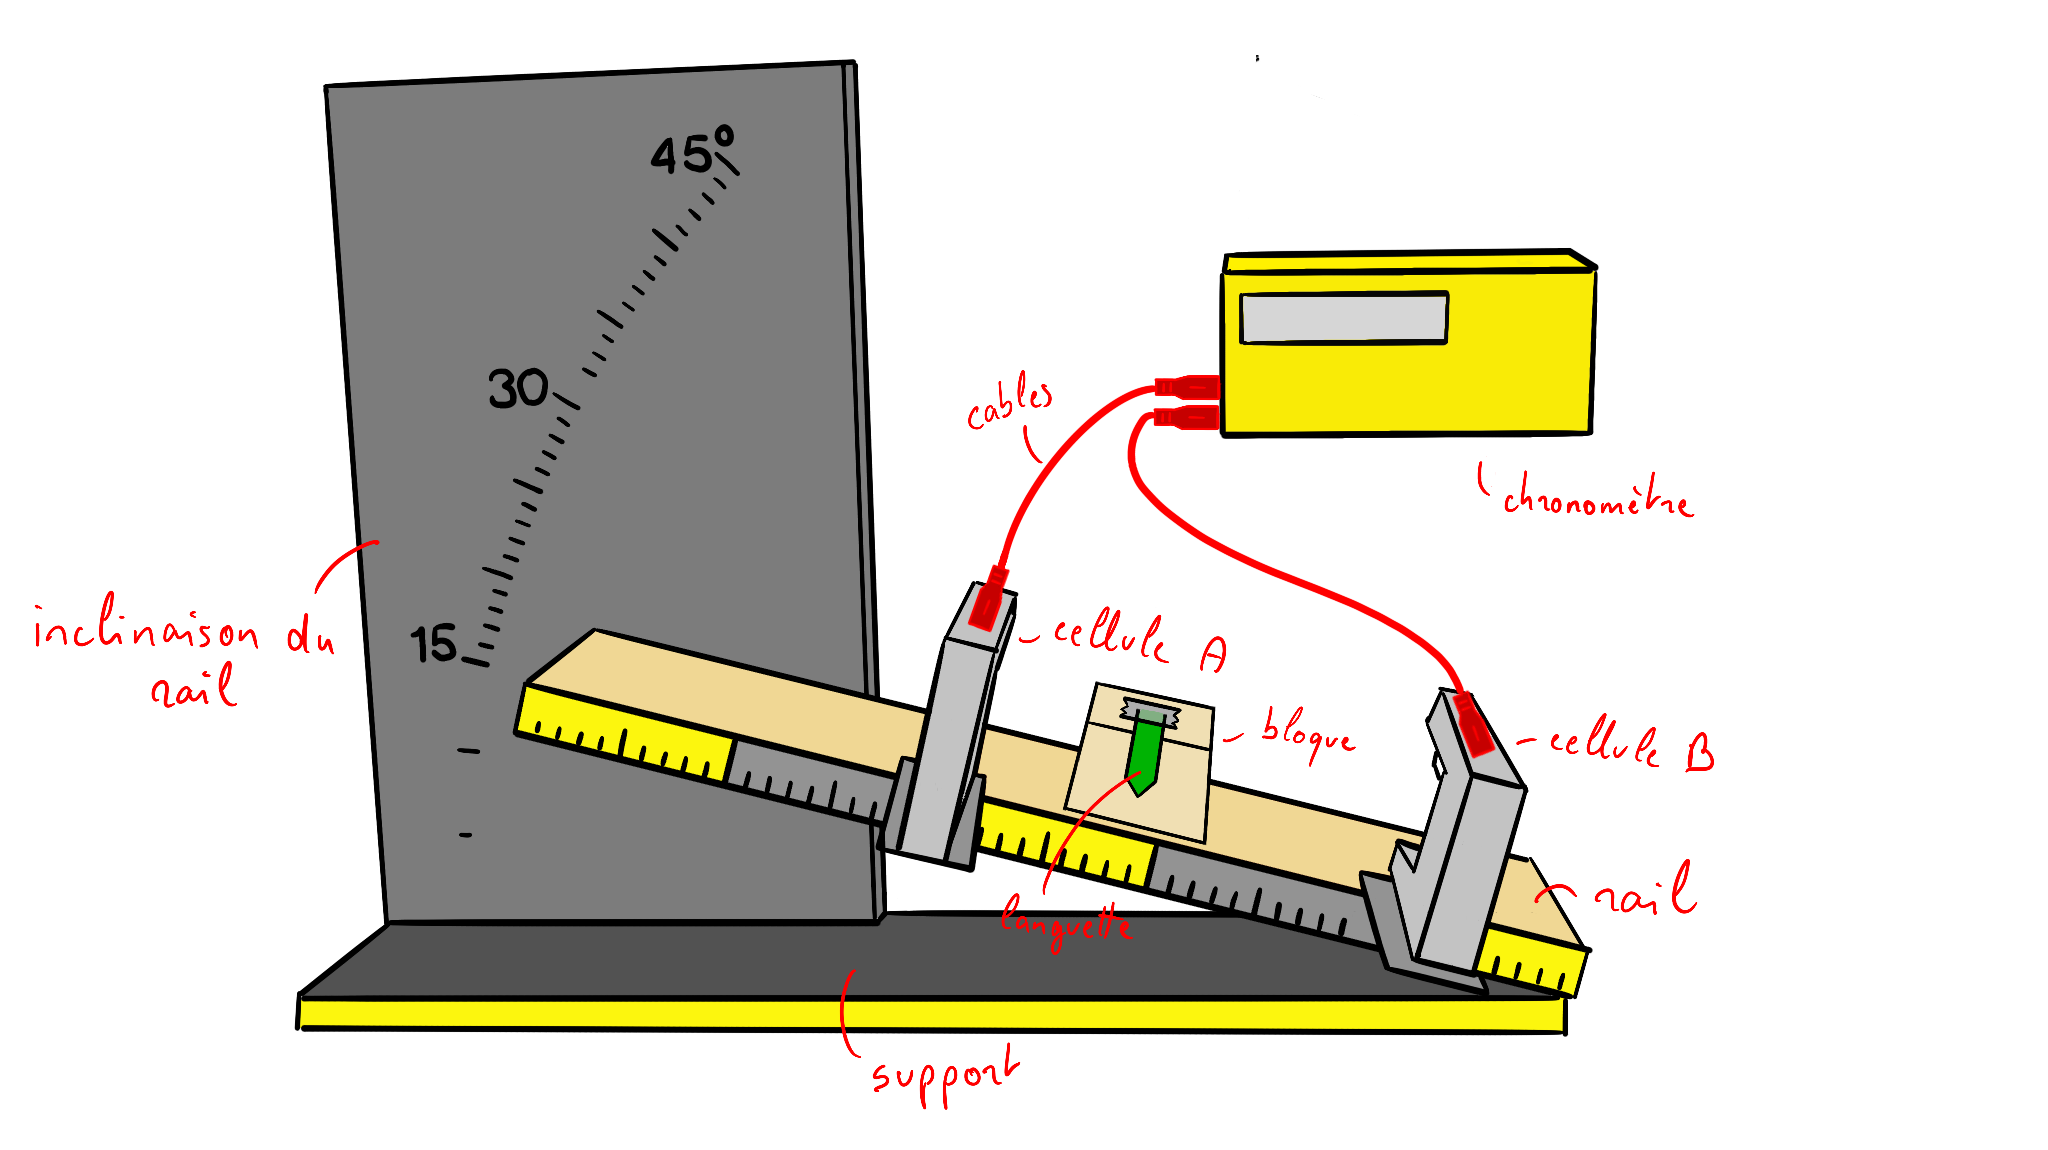
\includegraphics[scale=0.125]{dessin_exp.png}
\caption{Schéma de l'expérience}
\end{figure}
%materiel
\subsection{Matériel utilisé}
\begin{itemize}
\item[•] Support
\item[•] Rail
\item[•] 2 cellules (nommées A et B)
\item[•] Languette
\item[•] Bloque en bois avec des faces vernis de papier de vert (émeri), plastique ou sans substance
\item[•] Rapporteur d’angle
\item[•] Câbles
\item[•] Chronomètre
\item[•] Support pour incliner le rail
\end{itemize}

%demarche
\subsection{Démarche expérimentale}
\begin{enumerate}
\item Assembler le matériel nécessaire à la procédure de l’expérience: brancher les câbles, scotcher la languette sur une face du bloque en bois, choisir la matière de la piste et régler son angle.
\item Préparer le chronomètre (bien veiller que les cellules A et B sont en marche).
\item Lâcher le bout en bois en ayant la languette regardant la direction des capteurs sans donner un coup d’avance comme cela peut fausser les résultats.
\item Noter les résultats obtenus, puis recommencer avec une matière ou angle différent.
\end{enumerate}

%------------------------------------------------

\section{Présentation des résultats}
\subsection{Mesures}
Ci-dessous les mesures prises lors de l'expérience.
\begin{table}[H]
\centering

%bois-bois
\caption{Bois sur Bois}
\begin{tabular}{|c|c|c|c|}
\hline
Angles [°] & $t_a$ [s] & $t_b$ [s] & $t_{ab}$ [s] \\
\hline \hline
15 & - & - & - \\
\hline
20 & 0.0668 & 0.0373 & 0.7123 \\
\hline
25 & 0.0461 & 0.0265 & 0.4912 \\
\hline
30 & 0.0394 & 0.0174 & 0.3617 \\
\hline
35 & 0.0307 & 0.0140 & 0.2933 \\
\hline
40 & 0.0260 & 0.0121 & 0.2517 \\
\hline
45 & 0.0274 & 0.0112 & 0.2436 \\
\hline
\end{tabular}
\label{table:mesurebb}

%bois-plastique
\caption{Bois sur plastique}
\begin{tabular}{|c|c|c|c|}
\hline
Angles [°] & $t_a$ [s] & $t_b$ [s] & $t_{ab}$ [s] \\
\hline \hline
15 & - & - & - \\
\hline
20 & 0.2131 & 0.0919 & 2.1748 \\
\hline
25 & 0.0615 & 0.0256 & 0.5720 \\
\hline
30 & 0.0427 & 0.0186 & 0.4029 \\
\hline
35 & 0.0314 & 0.0149 & 0.3119 \\
\hline
40 & 0.0299 & 0.0129 & 0.2804 \\
\hline
45 & 0.0280 & 0.0115 & 0.2542 \\
\hline
\end{tabular}
\label{table:mesurebp}

%plastique-plastique
\caption{Plastique sur plastique}
\begin{tabular}{|c|c|c|c|}
\hline
Angles [°] & $t_a$ [s] & $t_b$ [s] & $t_{ab}$ [s] \\
\hline \hline
15 & - & - & - \\
\hline
20 & - & - & - \\
\hline
25 & 0.0695 & 0.0462 & 0.8154 \\
\hline
30 & 0.0463 & 0.0238 & 0.4741 \\
\hline
35 & 0.0362 & 0.0178 & 0.3744 \\
\hline
40 & 0.0307 & 0.0144 & 0.3015 \\
\hline
45 & 0.0279 & 0.0127 & 0.2675 \\
\hline
\end{tabular}
\label{table:mesurepp}

%emeri-emeri
\caption{Émeri sur émeri}
\begin{tabular}{|c|c|c|c|}
\hline 
Angles [°] & $t_a$ [s] & $t_b$ [s] & $t_{ab}$ [s] \\
\hline \hline
15 & - & - & - \\
\hline
20 & 0.0824 & 0.0361 & 0.7492 \\
\hline
25 & 0.0451 & 0.0204 & 0.4238 \\
\hline
30 & 0.0361 & 0.0158 & 0.3366 \\
\hline
35 & 0.0331 & 0.0153 & 0.3087 \\
\hline
40 & 0.0249 & 0.0117 & 0.2433 \\
\hline
45 & 0.0281 & 0.0109 & 0.2416 \\
\hline
\end{tabular}
\label{table:mesureee}

\end{table}

\subsection{Conversion des mesures}
La conversion des [°] en $[rad]$ pour faciliter l'utilisation des logiciels.
\begin{table}[H]
\centering
\caption{Angles en unité SI}
\begin{tabular}{|l|l|}
\hline
Angles [°] & Angles [rad] \\
\hline \hline
15 & 0.262 \\
\hline
20 & 0.349 \\
\hline
25 & 0.436 \\
\hline
30 & 0.524 \\
\hline
35 & 0.611 \\
\hline
40 & 0.698 \\
\hline
45 & 0.785 \\
\hline
\end{tabular}
\label{table:angle}
\end{table}

\subsection{Calculs}
Ici sont noté les résultats des calculs de vitesse et d'accélération, ainsi que celle des forces de frottement et de soutient.
\subsubsection*{Vitesses et accélérations}
\begin{table}[H]
\centering
\caption{Bois sur bois}
\begin{tabular}{|c|c|c|c|}
\hline
Angle [°] & $v_a$ $\left[ \frac{m}{s} \right]$ & $v_b$ $\left[ \frac{m}{s} \right]$ & $a_{ab}$ $\left[ \frac{m}{s^2} \right]$ \\
\hline \hline
15 & - & - & - \\
\hline
20 & 0.299 & 0.536 & 0.332 \\
\hline
25  & 0.434 & 0.755 & 0.653 \\
\hline
30 & 0.508 & 1.149 & 1.774 \\
\hline
35 & 0.651 & 1.429 & 2.650 \\
\hline
40 & 0.769 & 1.653 & 3.511 \\
\hline
45 & 0.730 & 1.786 & 4.334 \\
\hline
\end{tabular}
\label{table:v-abb}

\caption{Bois sur plastique}
\begin{tabular}{|c|c|c|c|}
\hline
Angle [°] &$v_a$ $\left[ \frac{m}{s} \right]$ & $v_b$ $\left[ \frac{m}{s} \right]$ & $a_{ab}$ $\left[ \frac{m}{s^2} \right]$ \\
           \hline \hline
15        &- & - & - \\
           \hline
20        &0.094 & 0.218 & 0.057 \\
           \hline
25        &0.325 & 0.781 & 0.797 \\
           \hline
30        &0.468 & 1.075 & 1.506 \\
           \hline
35        &0.637 & 1.342 & 2.261 \\
           \hline
40        &0.669 & 1.550 & 3.144 \\
           \hline
45        &0.714 & 1.739 & 4.032 \\
           \hline
\end{tabular}
\label{table:v-abp}
\end{table}

\begin{table}[H]
\centering
\caption{Plastique sur plastique}
\begin{tabular}{|c|c|c|c|}
\hline
Angle [°] &$v_a$ $\left[ \frac{m}{s} \right]$ & $v_b$ $\left[ \frac{m}{s} \right]$ & $a_{ab}$ $\left[ \frac{m}{s^2} \right]$ \\
           \hline \hline
15        &- & - & - \\
           \hline
20        &- & - & - \\
           \hline
25        &0.288 & 0.433 & 0.178 \\
           \hline
30        &0.432 & 0.840 & 0.861 \\
           \hline
35        &0.552 & 1.124 & 1.525 \\
           \hline
40        &0.651 & 1.389 & 2.446 \\
           \hline
45        &0.717 & 1.575 & 3.207 \\
           \hline
\end{tabular}
\label{table:v-app}

\caption{Émeri sur émeri}
\begin{tabular}{|c|c|c|c|}
\hline
Angle [°] &$v_a$ $\left[ \frac{m}{s} \right]$ & $v_b$ $\left[ \frac{m}{s} \right]$ & $a_{ab}$ $\left[ \frac{m}{s^2} \right]$ \\
           \hline \hline
15        &- & - & - \\
           \hline
20        &0.243 & 0.554 & 0.416 \\
           \hline
25        &0.443 & 0.980 & 1.267 \\
           \hline
30        &0.554 & 1.266 & 2.115 \\
           \hline
35        &0.604 & 1.307 & 2.277 \\
           \hline
40        &0.803 & 1.709 & 3.725 \\
           \hline
45        &0.712 & 1.835 & 4.649 \\
           \hline
\end{tabular}
\label{table:v-aee}
\end{table}

\subsubsection*{Accélération des forces}
\begin{table}[H]
\centering
\caption{Bois sur bois}
\begin{tabular}{|c|c|c|}
\hline
Angle [°] & $F_f$ $\left[ \frac{N}{Kg} \right]$ &$S$ $\left[ \frac{N}{Kg} \right]$ \\
           \hline \hline
15        &- & 9.476 \\
           \hline
20        &3.023 & 9.218 \\
           \hline
25        &3.493 & 8.891 \\
           \hline
30        &3.131 & 8.496 \\
           \hline
35        &2.977 & 8.036 \\
           \hline
40        &2.795 & 7.515 \\
           \hline
45        &2.603 & 6.937 \\
           \hline
\end{tabular}
\label{table:v-abb}

\caption{Bois sur plastique}
\begin{tabular}{|c|c|c|}
\hline
Angle [°] & $F_{f}$ $\left[ \frac{N}{Kg} \right]$ &$S$ $\left[ \frac{N}{Kg} \right]$ \\
           \hline \hline
15        &- & 9.476 \\
           \hline
20        &3.298 & 9.218 \\
           \hline
25        &3.349 & 8.891 \\
           \hline
30        &3.399 & 8.496 \\
           \hline
35        &3.365 & 8.036 \\
           \hline
40        &3.162 & 7.515 \\
           \hline
45        &2.905 & 6.937 \\
           \hline
\end{tabular}
\label{table:v-abp}

\end{table}

\begin{table}[H]
\centering
\caption{Plastique sur plastique}
\begin{tabular}{|c|c|c|}
\hline
Angle [°] & $F_{f}$ $\left[ \frac{N}{Kg} \right]$  &$S$ $\left[ \frac{N}{Kg} \right]$\\
           \hline \hline
15        &- & 9.476 \\
           \hline
20        &- & 9.218 \\
           \hline
25        &3.968 & 8.891 \\
           \hline
30        &4.044 & 8.496 \\
           \hline
35        &4.101 & 8.036 \\
           \hline
40        &3.860 & 7.515 \\
           \hline
45        &3.729 & 6.937 \\
           \hline
\end{tabular}
\label{table:v-app}

\caption{Émeri sur émeri}
\begin{tabular}{|c|c|c|}
\hline
Angle [°] & $F_{f}$ $\left[ \frac{N}{Kg} \right]$ &$S$ $\left[ \frac{N}{Kg} \right]$ \\
           \hline  \hline
15        &- & 9.476 \\
           \hline
20        &2.940 & 9.218 \\
           \hline
25        &2.879 & 8.891 \\
           \hline
30        &2.790 & 8.496 \\
           \hline
35        &3.350 & 8.036 \\
           \hline
40        &2.581 & 7.515 \\
           \hline
45        &2.288 & 6.937 \\
           \hline
\end{tabular}
\label{table:v-aee}
\end{table}

\subsection{Coefficient de frottement}
Finalement, voici les coefficients de frottements obtenus :
\begin{table}[H]
\centering
\caption{Bois sur bois}
\begin{tabular}{|c|c|}
\hline
Angle [°] &$\mu$ \\
           \hline   \hline
15        &- \\
           \hline
20        &0.328 \\
           \hline
25        &0.393 \\
           \hline
30        &0.368 \\
           \hline
35        &0.370 \\
           \hline
40        &0.372 \\
           \hline
45        &0.375 \\
           \hline
\end{tabular}
\label{table:coeffbb}

\caption{Bois sur plastique}
\begin{tabular}{|c|c|}
\hline
Angle [°] &$\mu$ \\
           \hline   \hline
15        &- \\
           \hline
20        &0.358 \\
           \hline
25        &0.377 \\
           \hline
30        &0.400 \\
           \hline
35        &0.419 \\
           \hline
40        &0.421 \\
           \hline
45        &0.419 \\
           \hline
\end{tabular}
\label{table:coeffbp}
\end{table}

\begin{table}
\centering
\caption{Plastique sur plastique}
\begin{tabular}{|c|c|}
\hline
Angle [°] &$\mu$ \\
           \hline   \hline
15        &- \\
           \hline
20        &- \\
           \hline
25        &0.446 \\
           \hline
30        &0.476 \\
           \hline
35        &0.510 \\
           \hline
40        &0.514 \\
           \hline
45        &0.538 \\
           \hline
\end{tabular}
\label{table:coeffpp}

\caption{Émeri sur émeri}
\begin{tabular}{|c|c|}
\hline
Angle [°] &$\mu$ \\
           \hline   \hline
15        &- \\
           \hline
20        &0.319 \\
           \hline
25        &0.324 \\
           \hline
30        &0.328 \\
           \hline
35        &0.417 \\
           \hline
40        &0.343 \\
           \hline
45        &0.330 \\
           \hline
\end{tabular}
\label{table:coeffee}
\end{table}

Si l'on prend la moyenne des valeurs obtenues - avec comme incertitude l'écart le plus grand entre la moyenne et la valeur des tableaux et l'incertitude relative, on a :
\begin{itemize}
\item Bois sur bois : $\mu \approx 0.368 \pm 0.040$ ou $10.85\%$
\item Bois sur plastique : $\mu \approx 0.399 \pm 0.041$ ou $10.28\%$
\item Plastique sur plastique : $\mu \approx 0.497 \pm 0.050$ ou $10.16\%$
\item Émeri sur émeri : $\mu \approx 0.344 \pm 0.073$ ou $21.33\%$
\end{itemize}

%------------------------------------------------

\section{Discussion des résultats}
Les résultats obtenus sont satisfaisant. En effet, on peut constater que le coefficient de frottement varie quand même d'une mesure à l'autre, mais reste autour d'une certaine moyenne. Comme on peut le voir sur chaque tableau, pour un angle de 15 [°], les blocs ne glissent pas, lorsque pour un angle de 20 [°], seul le "plastique-plastique" ne bougeait pas, ce qui laissait tout de suite penser que le coefficient de frottement serait plus grand, ce qui est confirmé par les résultats. De plus, on constate que l' "émeri-émeri" est la combinaison avec le moins de frottement dans notre expérience, mais également la mesure avec le plus d'incertitude ($\sim 20 \%$ contre $\sim 10 \%$ pour le reste). Ces incertitudes assez élevées, mais pas déraisonnable pour autant, peuvent s'expliquer par l'imprécision dans la mise en place de la mesure, ainsi que sa propagation au fil des calculs. De fait, lors de l'expérience, la mise en place de la rampe sur le bon angle n'était pas d'une précision à tout épreuve au vu du matériel à disposition. Ensuite, la manière dont le bloc de bois glissait sur la rampe, avec par moment des comportements étrange, comme de légers à-coup ou la nécessiter de toucher le bloc afin de le mettre en mouvement (pour certaines matières lorsque l'angle est trop faible), mais ces raison sont très secondaire vis-à-vis de la première exprimée.

%------------------------------------------------

\section{Conclusion}
En conclusion on peut voir clairement que la masse ne joue pas dans le système comme supposée au début car elle s'annule dans les équations, deuxièmement en regardant les résultats on constate que le coefficient de frottement cinétique ne dépend que des surfaces mises en jeu et que l'angle n'influence en aucun cas dans ce dernier également correcte vis-à-vis des suppositions du début. On remarque également que plus le coefficient de frottement est grand moins le bloc aura tendance à bouger. Ceci s'applique à toutes les surfaces pas seulement celle testée au dessus. L'expérience n'est pas parfaitement précise car le bloc aurait pus être poussé ou retenus au lancement car il est sûrement partit avec de la vitesse, l'angle aurait pus être mal mis, la surface pas égale sur toute la longueur, etc. Néanmoins, les résultats sont satisfaisant et ont permis de confirmer les hypothèses.

\end{document}
